\documentclass[ams]{U-AizuGT}
\usepackage{pifont}
\usepackage[dvipdfmx]{graphicx}
\usepackage{cite}
\hyphenpenalty=10000\relax
\exhyphenpenalty=10000\relax
\sloppy

\bibliographystyle{ieicetr}

\author{Kaisei Konno}
\studentid{s1230051}
\supervisor{Kazuyoshi Mori}
\title{Learning System to Visualize Hierarchical Structure of High school Mathematics on iOS [abstracted by Ryoma Okuda s1270174]}

\begin{document}
	\maketitle
	\section{abstract}
		教育は常日頃促進している。教科書だけで学ぶのだけではなく、ICT教育を取り入れることもできる。今回はiOS用の教育用アプリを製作した。

	\section{Introduction}
		\subsection{Logically in School}
		高校の教育では問題を論理的に考えるということが答えをみただけで理解することができない生徒が多々存在する。

    最近ではICT教育はFigure 1のように、実際に教育で使われていることがわかっている。

    ICT環境を使うことによって、実物の教科書を使わずにタブレットを用いている。用いることによって生徒と教師間のコミュニケーションが容易になったり、書類の作成が比較的容易になる。

    この研究ではiOSアプリ製作によって、生徒の論理的に考える力を養うことを目標とした。

    \begin{figure}[htb]
      \centering
      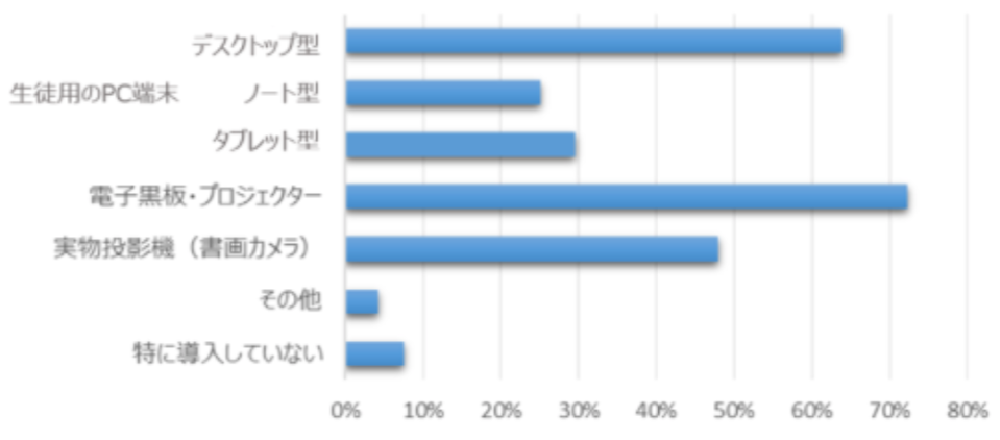
\includegraphics[width=6cm]{img/figure1.pdf}
      \caption{The use situation ICT in field of education}
      \label{fig:ict}
    \end{figure}


		\subsection{iOS}
			iOSはApple社がモバイル端末向けに開発したOSで、iPhone, iPod Touch, iPadなどに搭載されている。

      \begin{figure}[htb]
        \centering
        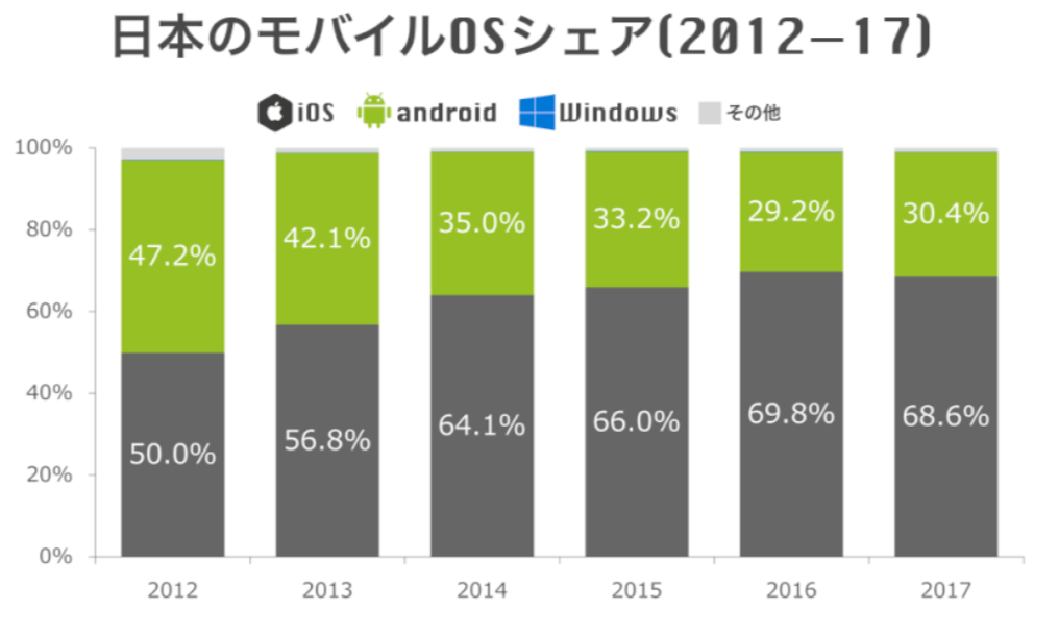
\includegraphics[width=6cm]{img/figure2.pdf}
        \caption{OS share in Japan}
        \label{fig:ict}
      \end{figure}

      Figure 2を見ると、日本では多くの人がAndroid端末よりiOS端末を使用している。

	\section{Development environment}
		\subsection{iOS developer university program}
iOS用のアプリケーションを開発するには、iOS developer university programという物に加入する必要がある。

\subsection{Xcode}

XcodeはmacOSに初期搭載されているフリーソフトウェアで、今回はStoryboardを使用してUIを作成した。

\subsection{Swift}

SwiftはiOS, macOS, Linuxで動くプログラミング言語である。

\subsection{Storyboard}

Sotryboardは狭いモバイル向けアプリケーションで、よりみやすいUIを開発するための環境です。

\subsection{Mathjax}

Mathjaxはウェブ上で特定の環境で記述された数式を表示するjavascriptのライブラリのことである。今回はこのMathjaxを計算能力向上の目的で使用した。

	\section{How this application move}

このアプリケーションを利用することによって、二項定理、三角関数、数学的帰納法が学習できる。(Figure 3,4,5を参照)

\section{Conclusion and Future works}

このアプリケーションを製作することにより、ICTを用いて学習した方が効率が良いということがわかった。

しかし、このアプリケーションでは学べる項目が少ないため、多くのことは学べない。高校で学ぶ範囲の数学を全て追加していく必要がある。

数学においては答えは一つだが、導き方は多数ある。故に解き方も多数用意する必要がある。



\subsection{References}

     ICT: https://hnavi.co.jp/knowledge/blog/ict/
     文部科学省 高等学校学習指導要領解説 数学編
     教育 ICT ガイドブック 総務省: https://www.soumu.go.jp/main-content/000492552.pdf
     iOS: https://ja.wikipedia.org/wiki/iOS
     iOS developer program: https://developer,apple.com/jp/support/university/
     Xcode: https://developer.apple.com/jp/xcode/
     Storyboard: https://iosdev.wiki.fc2.com/wiki/storyboard/
     Swift:  https://www.apple.com/jp/swift/
     mathjax: https://www.mathjax.org/
     \begin{figure}[htb]
       \centering
       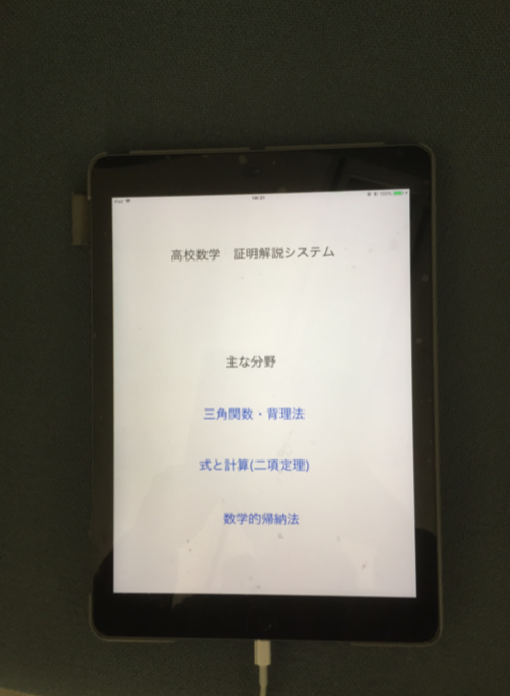
\includegraphics[width=6cm]{img/figure3.pdf}
       \caption{The photograph of the application of ios}
       \label{fig:ict}
     \end{figure}

     \begin{figure}[htb]
       \centering
       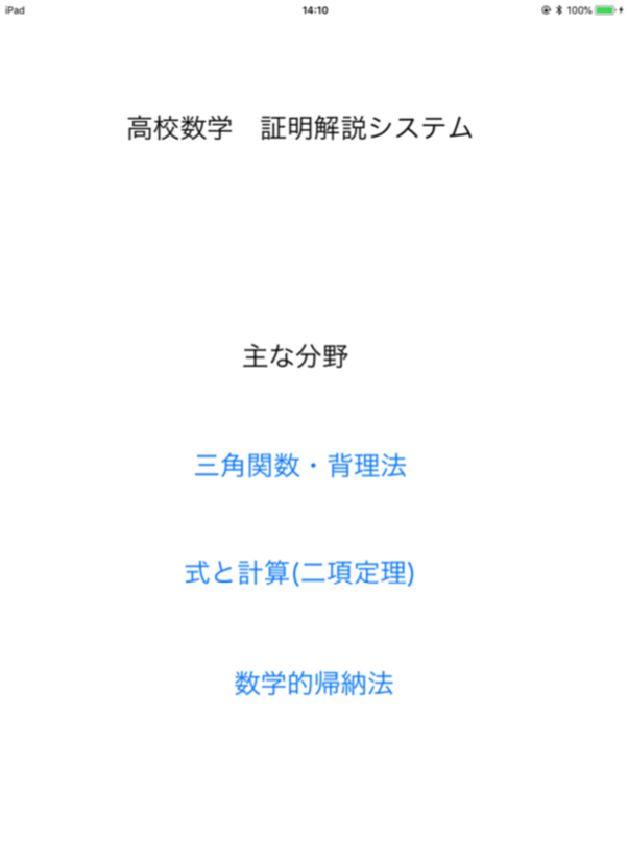
\includegraphics[width=6cm]{img/figure4.pdf}
       \caption{Top of this iOS application}
       \label{fig:ict}
     \end{figure}

     \begin{figure}[htb]
       \centering
       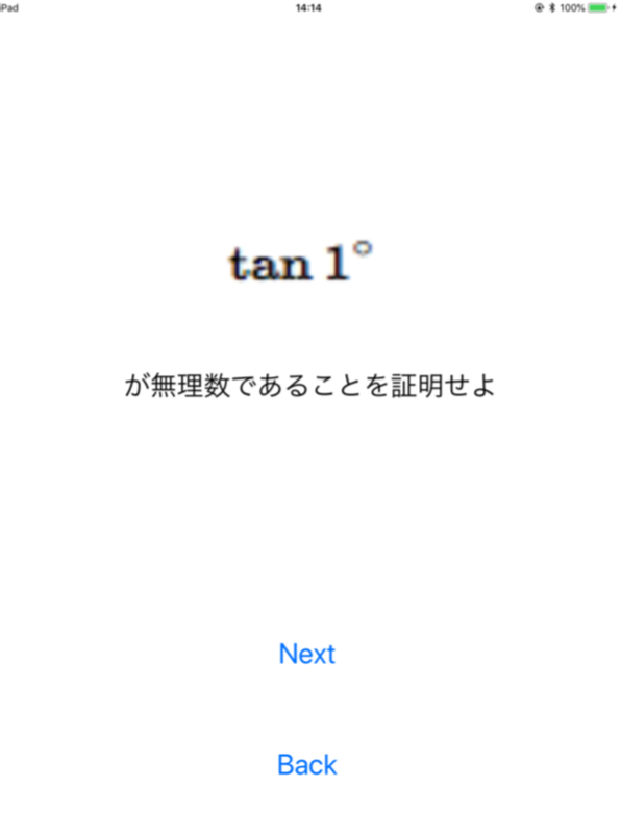
\includegraphics[width=6cm]{img/figure5.pdf}
       \caption{三角関数}
       \label{fig:ict}
     \end{figure}

	\bibliography{biblist}

\end{document}
